\section{Results}
\subsection{CO emission maps}

\begin{figure*}[htbp]
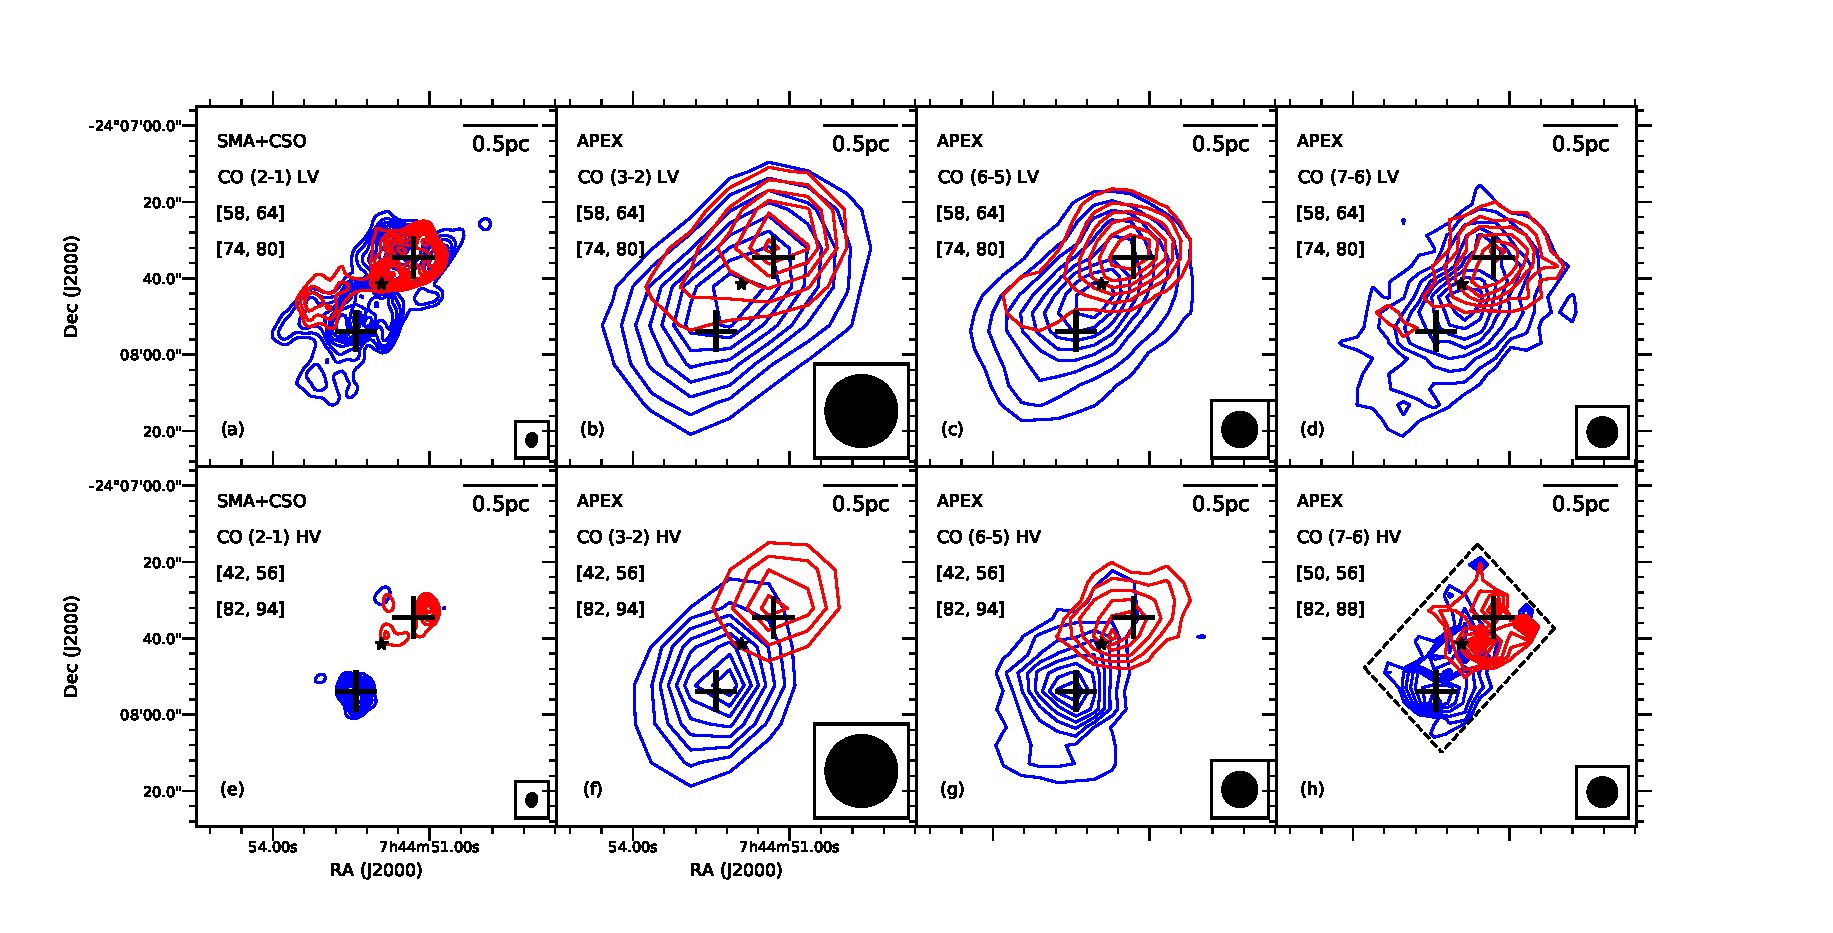
\includegraphics[scale=.65]{./fig/ori_contourall.eps}
\caption{(a)-(d) Low-velocity CO J = 2-1, 3-2, 6-5, 7-6 emissions, integrated from 58 to 64 km s$^{-1} $ for the blueshifted lobe (blue) and from 74 to 80 km s$^{-1}$ for the redshifted lobe (red); (e)-(f) High-velocity CO J = 2-1, 3-2 emissions,  integrated from 42 to 56 km s$^{-1} $ for the blueshifted lobe (blue) and from 82 to 94 km s$^{-1}$ for the redshifted lobe (red); (g) High-velocity CO J = 6-5 emission, integrated from 44 to 56 km s$^{-1} $ for the blueshifted lobe (blue) and from 82 to 92 km s$^{-1}$ for the redshifted lobe (red) (h) High-velocity CO J = 7-6 emission, integrated from 46 to 56 km s$^{-1} $ for the blueshifted lobe (blue) and from 82 to 90 km s$^{-1}$ for the redshifted lobe (red). For (a)-(g), the contour levels start from 20\% and continue at steps of 10\% of the peak emission. For (h), the contour levels start from 30\% and continue at steps of 10\% of the peak emission. Edge channels are masked out because of high noise levels. The black star marks the position of a H$_2$O maser spot which is associated with IRAS 07427-2400 \citep{2015PASJ...67...69S}. The beam of each observational dataset is shown in the lower right corner of each panel. \label{fig:figcontour}}
\end{figure*}

The CO 3-2, 6-5 and 7-6 emissions are detected (with obvious outflow signatures and with peak intensities $>$ 2 $\sigma_{rms}$) in velocity ranges from 42 km s$^{-1}$ to 94 km s$^{-1}$, 44 km s$^{-1}$ to 92 km s$^{-1}$, and 46 km s$^{-1}$ to 90 km s$^{-1}$, respectively. Figure \ref{fig:figcontour} shows the integrated low-velocity (LV) and high-velocity (HV) emissions of the four lines. The velocity ranges chosen to highlight the LV and HV components of the outflowing gas follow those in \citet{2009ApJ...696...66Q}, except that the channels with no detections were excluded for the HV component. The morphologies of the bipolar outflow seen in the emission from the CO 3-2, 6-5 and 7-6 lines are very similar. Due to the coarser angular resolution, the wide-angle structure seen in the higher resolution CO 2-1 image is not seen in the CO 3-2, 6-5, 7-6 maps.

\subsection{Physical conditions of the outflow}
\subsubsection{Methodology}

\begin{figure}[tbp]
\plotone{./fig/ratio.eps}
\caption{Ratios of the main-beam brightness temperatures of different CO lines at different velocities. Blue symbols denote the measurements from the blueshifted lobe, and red symbols the redshifted lobe. The $V_{\mathrm{outflow}}$ shown here is related to the cloud velocity $v_{\mathrm{cloud}}$ by the relation: $V_{\mathrm{outflow}}$ = $\mid$ $v_{\mathrm{outflow}}$ - $v_{\mathrm{cloud}}\mid$, where $v_{\mathrm{outflow}}$ is the outflow velocity with respect to the local standard of rest. \label{fig:figratio}}
\end{figure}

The physical conditions of the outflow can be constrained by comparing the observed line intensities with the results of statistical-equilibrium calculations. To study the four lines at the same spatial resolution, the CO 2-1, 6-5 and 7-6 maps were reconstructed with the same beam of the CO 3-2 map. The average rms noise levels are $\sim$0.004 K, $\sim$0.04 K and $\sim$0.1 K for the convolved CO 2-1, 6-5 and 7-6 data, respectively. For both lobes of the outflow, the CO line intensities were measured at roughly the peak positions of the HV components of the convolved CO maps (marked as two crosses in every panel of Figure \ref{fig:figcontour}), and were then used in the following analysis. Figure \ref{fig:figratio} shows the ratios of the main-beam brightness temperatures ($T_{\mathrm{mb}}$) of different CO lines as functions of velocity. The CO 7-6/6-5, 6-5/3-2, and 6-5/2-1 ratios are remarkably constant over a velocity range of $\sim 5-25$ km s$^{-1}$ with respect to the cloud velocity. In the analysis, we only used channels of $\le$ 60 km s$^{-1}$ and $\ge$ 74 km s$^{-1}$ to avoid contaminations from the ambient gas, and we excluded channels of $<$ 46 km s$^{-1}$ or $>$ 90 km s$^{-1}$ because of their low signal-to-noise ratios. The outflow emission was analyzed in each 2 km s$^{-1}$ bin. Considering that the $^{13}$CO 2-1 emission was only marginally detected in the outflowing gas with high sensitivity observations \citep{2009ApJ...696...66Q}, we assumed the four $^{12}$CO lines to be optically thin. In the optically thin case, the source size is degenerate with column density (see section \ref{section:density}). We didn't correct the observed line intensities for beam filling factors, so the derived CO column densities should be considered as beam-averaged values. In the calculation, errors on line intensities took into account both the calibration error and the rms noise. 
%(R.A., decl.)$_{J2000}$ = ($07^h44^m52^s.4, -24^d7^m53^s.8$) and (R.A., decl.)$_{J2000}$ = ($07^h44^m51^s.3, -24^d7^m34^s.6$)
%We note that the offsets of the peak positions are within $\sim$ 3$\arcsec$ for different lines at different velocities.
%The uncertainty of the observed intensity mainly consists of two parts: the calibration error and the rms noise. At low velocities, the calibration uncertainty dominates the intensity uncertainty, whereas the rms noise is dominant at high velocities. A combination of the rms noise and the calibration error $\sigma_{obs} = (\sigma_{cal}^2 + \sigma_{rms}^2)^{\frac{1}{2}}$ was used as the observational uncertainty in the belowing analyses.
%errors take into account both the rms noise and the calibration uncertainties.

\subsubsection{Rotation diagram analysis\label{subsec:RD}}

\begin{figure}[tbp]
\plotone{./fig/RD.eps}
\caption{A rotation diagram for CO at 84 km s$^{-1}$. The fitted line shows the Boltzmann distribution of the rotational populations. The line represents a rotational temperature of 48.5 K and a total column density of 2.0 $\times$ 10$^{15}$ cm$^{-2}$. The black solid circles show the data with error bars. \label{fig:figrd}}
\end{figure}

Firstly, we performed a simple rotation diagram (RD) analysis \citep{1999ApJ...517..209G} to estimate the excitation conditions of the outflowing gas under the assumption of local thermal equilibrium (LTE). The population of each energy level is given by 
\begin{equation}
N_{\mathrm{up}} = \frac{N_\mathrm{CO}}{Z} g_\mathrm{up} e^{-E_\mathrm{up}/kT_\mathrm{kin}},
\end{equation}
where $N_\mathrm{up}$ is the column density in the upper state, $g_\mathrm{up}$ the statistical weight of the upper state, $E_\mathrm{up}$ the upper energy level, $k$ the Boltzmann constant, and $Z$ is the partition function. The rotation diagram for CO at 84 km s$^{-1}$ is shown in Figure \ref{fig:figrd} as an example. The different energy levels are well reproduced by a single-component, indicating that the four transitions are probing the same volume of gas. Similar rotation diagram patterns with one gas component are found at other velocities. The derived gas temperature and CO column density as functions of the gas velocity are shown in Figure \ref{fig:figrelation}.

\subsubsection{Large velocity gradient analysis\label{subsec:LVG}}

\begin{figure*}[!tbp]
\gridline{\fig{./fig/chiimage_nco_paper.eps}{0.5\textwidth}{(a)}
        \fig{./fig/chiimage_nh2_paper.eps}{0.5\textwidth}{(b)}}
 \gridline{\fig{./fig/chiimage_tkin_paper.eps}{0.5\textwidth}{(c)}
      }
\caption{(a)-(c) The $\chi^2$ distribution at 84 km s$^{-1}$ in the [$T$, $n$], [$T$, $N$] and [$n$, $N$] planes, with the third parameter fixed to the value of the best fitting result at this velocity. The lower limit of gas density is 1.8 $\times$ 10$^{5}$ cm$^{-3}$. The best-fit solution is obtained for $T$ =  46.1 K and N = 2.2 $\times$ 10$^{15}$ cm$^{-2}$. The $\chi^2_{\mathrm{red}}$ of the best-fit solution is 1.00. The Solid white contours show the 1$\sigma$ confidence levels. \label{fig:figchi}}
\end{figure*}

Secondly, the non-LTE radiative transfer code RADEX \citep{2007A&A...468..627V} was used to better constrain the gas density ($n$), the kinetic temperature ($T$) and the CO column density ($N$) of the outflowing gas. RADEX employs the the LVG approximation. We built a large grid of LVG models varying the three parameters ($n$, $T$ and $N$), and obtained the best fitting results by minimizing the $\chi^2$ calculated from the observed intensities and the model intensities. With four lines observed and three parameters to constrain, our fitting had one degree of freedom. In Figure \ref{fig:figchi}, the fitting results at 84 km s$^{-1}$ are shown as examples of the distributions of $\chi^2$. Only one minimum of $\chi^2$ is found in the [$T$, $N$] plane. In the [$T$, $n$] and [$n$, $N$] planes, the $\chi^2$ distributions show that the gas is thermalized and no upper limits to the H$_2$ density could be derived, which confirms the LTE assumption of the rotation diagram analysis. Similar $\chi^2$ distribution patterns were found at other velocities. The best-fit solutions at different velocities are very close to the results of the rotation diagram (see Figure \ref{fig:figrelation}). The reduced $\chi^2$ ($\chi^2_{\mathrm{red}}$) of the best fitting results varies from 0.10 to 1.72 at different velocities. We derive the uncertainties of each parameter from the 1$\sigma$ confidence region in the 3D parameter space at the velocities where $\chi^2_{\mathrm{red}} \sim 1$ as the representative parameter uncertainties. The uncertainty of CO column densities is $\sim$ 10 \%. The 1$\sigma$ confidence range of the temperature is about 40 K - 60 K. And the gas density is $>$ 10$^5$ cm$^{-3}$ over the entire outflow. The modeling results also predict that the four transitions are optically thin in the outflowing gas, which is consistent with our assumptions. Figure \ref{fig:figsed} shows the comparison of the observed CO intensities with the LVG modeling results in each velocity bin. 
% Though the best-fitted $\chi^2_{\mathrm{red}}$ varies, the $\chi^2_{\mathrm{red}}$ distribution profiles show similarity in morphology at different velocities, indicating that the uncertainties of the fitted parameters may have similar levels at different velocities.

\subsubsection{$T$-$V$ and $N$-$V$ relations}

\begin{figure*}[!tbp]
\gridline{\fig{./fig/tv_paper.eps}{0.5\textwidth}{(a)}
          \fig{./fig/Nv_paper.eps}{0.5\textwidth}{(b)}
          }
\caption{$T$-$V$ and $N$-$V$ diagrams of the G240 outflow, estimated from the rotation diagram analysis (blue ``x'' markers for the blue lobe and red ``x'' markers for the red lobe) and the LVG analysis (blue open squares for the blue lobe and red open squares for the red lobe). \label{fig:figrelation}}
\end{figure*}

In Figure \ref{fig:figrelation}, the $T$-$V$ diagram shows that the gas is approximately isothermal with a gas temperature of $\sim$ 50 K, while the $N$-$V$ diagram shows that the CO column density in each 2 km s$^{-1}$ bin decreases from $\sim 2 \times 10^{16} $ cm$^{-2}$ at $\sim \pm$ 7 km s$^{-1}$ down to $\sim 4 \times 10^{14}$ cm$^{-2}$ at $\sim \pm$ 22 km s$^{-1}$. We compared the model intensities with line intensities measured at several different positions, and found that the modeling results are similar to those represented in Figure \ref{fig:figrelation}. Thus, a systematic bias of position offsets was excluded.
%Thus, we exclude the systematic bias from choices of positions for measuring the line intensities.




